

\chapter{General Trust Assessment Methodology  [By End of March] }
\label{chap:Trust_method}
\section{Role of the General Trust Assessment Methodology}
\label{sec:ch4_role}
This chapter introduces the \emph{General Trust Assessment Methodology} that serves as the conceptual backbone of this dissertation. The methodology is grounded in the Evidence-based \ac{TAF}, originally developed in the context of multi-agent systems within the Horizon Europe CONNECT project~\cite{connect_d31_taf}and also discussed in the 5GAA white paper on trust evaluation~\cite{5gaa_trust_whitepaper}. In this framework, trust is not assumed or statically assigned
but instead derived through a structured reasoning process that includes the generation of expressions, the collection of evidence, and the evaluation of these expressions.

The objective of this chapter is to abstract and generalize this evidence-based reasoning process so that it can be instantiated across different \ac{AI} contexts. While the technical mechanisms used to compute trust may vary across systems, the underlying reasoning process remains largely invariant. The methodology introduced here therefore provides a unified framework for structuring trust assessment problems and systematically deriving trust evaluations from observable evidence.

In the remainder of this dissertation, this general methodology will be instantiated in several distinct settings:

\begin{itemize}
    \item the trust assessment of neural network prediction calibration (\cref{chap:bb}),
    \item the evaluation of training dataset trustworthiness (\cref{chap:data}),
    \item the propagation of trust through neural network architectures using the PaTAS framework (\cref{chap:ptas}).
\end{itemize}

Although these application domains differ in their technical implementations, they share a common conceptual structure. In each case, a \emph{trustor} seeks to determine whether a specific trust proposition holds for a given entity or process, based on available evidence and within a particular contextual setting. The methodology presented in this chapter formalizes this common reasoning structure. In particular, it defines the sequence of steps required to construct a trust assessment and provides guidance on how each step can be operationalized in practice.

The methodology should therefore be understood as a generic trust reasoning engine. Subsequent chapters specialize this engine to particular trustworthiness properties and application domains, while preserving the same conceptual pipeline defined in this chapter.

\section{Core Concepts and Notation}
\label{sec:ch4_core_concepts}
The terminology follows the principles of the \ac{TAF}, which adopts \acf{SL} as the formal reasoning framework for representing and propagating trust. The notation introduced here is therefore consistent with \ac{SL} representations.

% \subsection{Trustor, Trustee, and Trust Proposition}

Trust assessment is inherently relational. A trust evaluation is always performed from the perspective of a \emph{trustor} with respect to a well-defined \emph{trust proposition} encoding a specific \emph{trustee}.

\begin{definition}[Trust Proposition]
A trust proposition is a declarative statement about a property of a trustee
that can be evaluated as satisfied or not satisfied based on available
evidence.
\end{definition}

Formally, let $E$ denotes the trustee and $P$ a
trustworthiness property of interest, such as accuracy, integrity, representativeness, or calibration. The trust proposition is denoted by
\[
\mathcal{T}(E, P)
\]
and represents the statement: ``Entity $E$ satisfies property $P$''

Trust propositions may take different forms:
\begin{itemize}
    \item \textbf{Simple}, when they refer to a single assessable property.
    \item \textbf{Composite}, when they are constructed as logical combinations
    of several simple propositions.
\end{itemize}

Composite trust propositions are typically expressed using logical operators such as conjunction, disjunction, and negation. For example, a composite proposition may take the form

\[
\mathcal{T} = \mathcal{T}_1 \wedge \mathcal{T}_2
\]

where each $T_i$ represents independent simple proposition.



% Each of these properties can be evaluated using separate evidence sources
% before being combined to assess the overall trust proposition.

% \subsection{\acf{ATL}}


% \subsection{Trust Sources and Evidence}


\begin{definition}[\aclu{ATO}]
An \acf{ATO} is a trust opinion associated with a simple trust proposition for which the trustor can directly observe or collect evidence about the trustee. In this case, the trustor maintains a direct evidential relationship
with the trustee and can therefore quantify trust based on observable
evidence.
\end{definition}
In the methodology, trust assessment of \ac{ATO} relies on evidence collected from \emph{trust sources}.

\begin{definition}[Trust Source]
A trust source is any entity, mechanism, or process that provides evidence
relevant to the evaluation of a trust proposition.
\end{definition}

Trust sources may include:

\begin{itemize}
    \item direct observations performed by the trustor,
    \item measurements from sensors or monitoring systems,
    \item reports or certifications provided by third parties,
    \item historical performance records,
    \item reputation information,
    \item outputs of analytical or verification mechanisms.
\end{itemize}


The outcome of the overall process is referred to as the \emph{\acf{ATL}}.
\begin{definition}[\aclu{ATL}]
The \ac{ATL} is the quantified trust opinion assigned by the trustor to a
trust proposition based on the available evidence and the selected evaluation
formalism.
\end{definition}

In this dissertation, the \ac{ATL} is represented using a subjective binomial
opinion:

\[
\omega = (t, d, u)
\]

where $t$ denotes the trust mass (belief of the binomial opinion), $d$ denotes distrust (disbelief of the binomial opinion), and $u$ represents uncertainty. This representation allows the trust assessment to capture not only whether the trustor should trust the proposition, but also the degree of confidence associated with that assessment.

For clarity, the main elements introduced in this section are summarized in \cref{tab:trust_notation}.

\begin{table}[h]
\centering
\begin{tabular}{ll}
\toprule
Symbol & Description \\
\midrule
$A$ & Trustor (entity performing the trust assessment) \\
$E$ & Trustee (entity whose property is being evaluated) \\
$P$ & Trustworthiness property \\
$\mathcal{T}(E,P)$ & Trust proposition stating that entity $E$ satisfies property $P$ \\
$\omega=(t,d,u)$ & trust opinion with belief $b$, disbelief $d$, and uncertainty $u$ \\
\ac{ATO} & \aclu{ATO} associated with a simple proposition \\ 
\ac{ATL} & outcome of the assessment\\
\bottomrule
\end{tabular}
\caption{Notation used in the general trust assessment methodology.}
\label{tab:trust_notation}
\end{table}

These concepts provide the conceptual foundation for the trust assessment process introduced in the next section.

\section{The Trust Assessment Process}
\label{sec:ch4_three_phase}

Having introduced the core concepts and notation, we now present the
general trust assessment process. This process follows the \ac{TAF} methodology and consists of three sequential phases:

\begin{enumerate}
    \item Expression Generation that sometimes necessitate a \ac{STN}. The expression consists in operations between \acp{ATO}.
    \item \acp{ATO} Quantification
    \begin{enumerate}
        \item Identify trust sources and Collect Evidence for each proposition
        \item Quantify the trust opinion for each trust source using the most appropriate quantification method.
        \item Derive the \ac{ATO}
    \end{enumerate}
    \item Expression Evaluation
\end{enumerate}

Each phase is described in detail below.

\subsection{Phase I: Expression Generation}
\label{subsec:ch4_expression_generation}

The purpose of this phase is to formally construct an expression that captures the relationships required to evaluate a given trust proposition.

Let $\mathcal{T}$ denote a trust proposition. In general, $\mathcal{T}$ is not directly measurable. Instead, it must be decomposed into a set of simple propositions that correspond to individually assessable properties:
\[
\mathcal{T} = f(\mathcal{T}_1, \mathcal{T}_2, \dots, \mathcal{T}_n)
\]

where $f(\cdot)$ is based on logical composition operators.

As an illustrative example, consider the trust proposition stating that a training dataset $\mathcal{D}$ is reliable. This proposition may be expressed as the conjunction of several simple propositions:

\[
\mathcal{T} =
\mathcal{T}(\mathcal{D},\text{label-accurate})
\wedge
\mathcal{T}(\mathcal{D},\text{measurement-accurate})
\wedge
\mathcal{T}(\mathcal{D},\text{representative})
\]

where:
\begin{itemize}
    \item $\mathcal{T}(\mathcal{D},\text{label-accurate})$ states that the dataset labels are accurate,
    \item $\mathcal{T}(\mathcal{D},\text{measurement-accurate})$ states that the feature measurements are accurate,
    \item $\mathcal{T}(\mathcal{D},\text{representative})$ states that the dataset adequately represents the target population.
\end{itemize}

This decomposition is critical but inherently subjective, as it depends on the judgment of the analyst defining the trust model. If relevant properties are omitted, the resulting \ac{ATL} may not accurately reflect the true trustworthiness of the evaluated entity. Conversely, excessive decomposition may introduce unnecessary complexity and additional sources of uncertainty. The level of granularity must therefore be aligned with the objectives and context of the trust assessment.

Once the proposition $\mathcal{T}$ has been decomposed, a \ac{STN} is constructed in order to evaluate each of the resulting simple propositions. The objective is to express the trust in $\mathcal{T}_i$ as a combination of atomic trust opinion using well-defined \ac{SL} operators such as trust discounting and belief fusion. The resulting expression defines how evidence and intermediate opinions will later be propagated and combined.

Within the \ac{TAF}, the construction of these expressions is performed by the \emph{\acf{TLEE}}. The \ac{TLEE} analyzes a \ac{STN} with a simple trust proposition as the target and derives an expression composed of \acp{ATO} and \ac{SL} operators. This analysis process is referred to as \emph{\acf{TNA-SL}}. We discuss this approach in more detail in the next chapter (\cref{chap:tnasl}), where we also present improvements motivated by the limitations identified in the related work (\cref{chap:rw}). The resulting expression serves as the computational blueprint for the subsequent phases of the trust assessment process.

At the end of Phase I, the assessment is represented as a structured expression whose evaluation will produce the final \ac{ATL}.


\subsection{Phase II: \aclu{ATO} Quantification}
\label{subsec:ch4_atomic_quantification}

Once the expression has been defined in Phase I, the next phase
consists of quantifying the \acp{ATO} appearing in that expression.
This phase consists of the following steps:

\begin{enumerate}
    \item Identify trust sources and collect evidence.
    \item Quantify the trust opinion associated with each trust source using the collected evidence and the most appropriate quantification method.
    \item Derive the \ac{ATO} by combining the trust opinions provided by the different trust sources.
\end{enumerate}

The first step establishes the evidential basis of the atomic trust assessment,
while the remaining steps transform collected evidence into a subjective
trust opinion.

\subsubsection{Identification of Trust Sources and Evidence Collection}

When quantifying the \ac{ATO} associated with a proposition $P_i$, relevant trust sources must first be identified. Trust sources may include, for example, a monitoring component, a sensor error measurement module, a misbehavior detection mechanism, a verification module, a certification authority, or historical performance records. These sources typically provide direct evidence corresponding to observations made by the
trustor.

Evidence collected from trust sources may take different forms:
\begin{itemize}
    \item Binary outcomes such as pass or fail,
    \item Counts of successful and unsuccessful events,
    \item Continuous measurements,
    \item Confidence scores.
\end{itemize}

These evidence are then mapped into a structured representation consisting of:
\begin{itemize}
    \item positive evidence $r_x$,
    \item negative evidence $s_x$,
    \item and, in some cases, structured uncertainty parameters.
\end{itemize}
When countable, it is straightforward to map the evidence into \(r_x\) and \(s_x\). Otherwise, if the evidence is not directly countable, an appropriate interpretation scheme must be devised to convert raw inputs into usable evidence components. For instance, a misbehavior detection mechanism applied to a sensor may either detect misbehavior (negative evidence \(s_x\)) or detect no anomaly (positive evidence\(r_x\)), which provides directly countable evidence. In contrast, continuous measurements of sensor error may require thresholding, normalization, or
probabilistic transformation before being translated into evidence counts.
%%%%%%%%%%%



\subsubsection{Trust Opinion Quantification Model}

After evidence has been identified, structured and collected, the next step consists of quantifying the trust opinion associated with each trust source.

In general, trust opinion quantification can be performed using different models, each reflecting specific assumptions about how uncertainty should be handled. In addition to the Baseline-Prior Quantification method motivated by \cref{eq:beta_mapping_forward}, we introduce two additional quantification models: Evidence-Weighted Quantification and Constant-Uncertainty Quantification.

\begin{enumerate}

    \item \textbf{Baseline-Prior Quantification.}  
    In this model, uncertainty decreases as the total number of positive and negative evidence increases.
    \begin{equation}
    \label{eq:baseline_quant}
    \begin{aligned}
        b_x &= \frac{r_x}{W + r_x + s_x}, \quad
        d_x = \frac{s_x}{W + r_x + s_x}, \quad
        u_x = \frac{W}{W + r_x + s_x}
    \end{aligned}
    \end{equation}
    The default value for the non-informative prior weight \(W\) is 2.
    \item \textbf{Evidence-Weighted Quantification.}  
    This method introduces a weight $w_x$ to account for uncertainty in addition to positive and negative evidence. It is particularly relevant when the evidence itself is associated with an uncertainty score. The belief, disbelief, and uncertainty are computed as:

    \begin{equation}
    \label{eq:weight_quant}
    \begin{aligned}
        b_x = \dfrac{r_x}{w_x + r_x + s_x}, \quad
        d_x = \dfrac{s_x}{w_x + r_x + s_x}, \quad
        u_x = \dfrac{w_x}{w_x + r_x + s_x}.
    \end{aligned}
    \end{equation}

    \item \textbf{Constant-Uncertainty Quantification.}  
    Unlike the previous models, this method maintains a fixed uncertainty level $U$, regardless of the number of evidence points. This is useful when uncertainty is determined by factors external to the number of positive and negative evidence.

    The belief and disbelief are scaled using a normalization factor $\gamma$:

    \begin{equation}
    \label{eq:constant_quant}
    \begin{aligned}
        u_x = U, \quad
        \gamma = \dfrac{1-U}{r_x + s_x}, \quad
        b_x = \gamma r_x, \quad
        d_x = \gamma s_x
    \end{aligned}
    \end{equation}

\end{enumerate}

Each of these models provides a distinct approach to handling uncertainty. The choice of quantification model depends on the characteristics of the available evidence, and the semantics of uncertainty in the application context.

After quantifying the trust opinions associated with individual trust sources, the resulting opinions are aggregated to derive the \ac{ATO}. One possible approach is to combine them using \ac{SL} fusion operators.
%%%%%%%%%%%%%%


\subsection{Phase III: Expression Evaluation}
\label{subsec:ch4_expression_evaluation}
\begin{figure}[t]
\centering
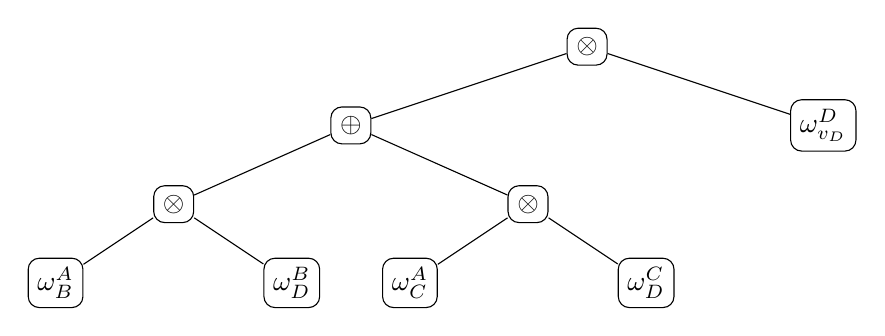
\begin{tikzpicture}[
level distance=1cm,
level 1/.style={sibling distance=6cm},
level 2/.style={sibling distance=4.5cm},
level 3/.style={sibling distance=3cm},
every node/.style={draw, rectangle, rounded corners, align=center},
edge from parent/.style={draw}
]

\node {$\otimes$}
    child {
        node {$\oplus$}
        child {
            node {$\otimes$}
            child { node {$\omega^A_B$} }
            child { node {$\omega^B_D$} }
        }
        child {
            node {$\otimes$}
            child { node {$\omega^A_C$} }
            child { node {$\omega^C_D$} }
        }
    }
    child {
        node {$\omega^D_{v_D}$}
    };

\end{tikzpicture}
\caption{Binary tree representation of the trust expression for the \ac{IMA} usecase}
\label{fig:trust_expression_tree}
\end{figure}

The final phase consists of evaluating the expression using the appropriate fusion and trust discounting operators once the values of the \acp{ATO} have been obtained. In our implementation, the expression is represented as a binary tree in which the leaves correspond to \acp{ATO} and the internal nodes correspond to \ac{SL} operators (\cref{fig:trust_expression_tree}). The evaluation of the expression is therefore performed recursively by propagating opinions from the leaves toward the root of the tree. After recursively evaluating the expression, a final subjective opinion is obtained. This opinion constitutes the \ac{ATL} associated with the original trust proposition $\mathcal{T}(E, P)$.


In summary, the trust assessment process can be performed in three phases:
\begin{enumerate}
    \item Generate an expression by decomposing the trust proposition into simple propositions and using \ac{TNA-SL} on \acp{STN} for each simple proposition.
    \item Quantify the \acp{ATO} in the expression by identifying relevant trust sources, collecting evidence, and applying an appropriate trust opinion quantification model.    
    \item Evaluate the expression using \ac{SL} operators such as fusion and trust discounting in order to derive the \ac{ATL}.
\end{enumerate}

This structured pipeline ensures that trust assessment remains transparent, reproducible, and adaptable across domains. In subsequent chapters, this generic process will be instantiated for dataset trustworthiness, calibration assessment, and \ac{NN} trust propagation.

\todo[inline]{Do I need to add an example? especially since as I said some chapters are already example. TAF paper with Nikos}